\documentclass[a4paper,11pt]{article}
\usepackage[utf8]{inputenc}
\usepackage{lastpage}
\usepackage{fancyhdr}
\usepackage[english]{babel}
\usepackage[a4paper,margin=1in]{geometry}
\usepackage{multirow}
\usepackage[table,xcdraw]{xcolor}
\usepackage{array}
\usepackage{graphicx}
\usepackage{caption}
\usepackage{ctable}
\usepackage{listings}
\usepackage[T1]{fontenc}
\usepackage{bigfoot} % to allow verbatim in footnote
\usepackage[numbered,framed]{matlab-prettifier}
\usepackage{amsmath}


\newcolumntype{L}[1]{>{\raggedright\let\newline\\\arraybackslash\hspace{0pt}}m{#1}}
\newcolumntype{C}[1]{>{\centering\let\newline\\\arraybackslash\hspace{0pt}}m{#1}}
\newcolumntype{R}[1]{>{\raggedleft\let\newline\\\arraybackslash\hspace{0pt}}m{#1}}

\newcommand\tab[1][4mm]{\hspace*{#1}}


%-------------------------------------------------------------------------------
% HEADER & FOOTER
%-------------------------------------------------------------------------------

\pagestyle{fancy}
\fancyhf{}
\setlength\headheight{15pt}
\fancyhead[L]{ Imaging Lab 8 }
\fancyhead[R]{Student ID: 100633486}
\fancyfoot[R]{Page \thepage\ of \pageref{LastPage}}


%-------------------------------------------------------------------------------
% TITLE PAGE
%-------------------------------------------------------------------------------

\begin{document}

\title{
	\Huge \textbf {Variational Methods}
    \\ [0.2cm]
	\LARGE Imaging Lab 8 - May, 2017
    \\ [0.5cm]
    \hrule
}

\date{}

\author{
		\Large Kamyar Nazeri \\
		\large Student ID: 100633486 }

\maketitle
\newpage

\section*{Total Variation Inpainting}
Inpainting is the process of reconstructing lost or deteriorated parts of images; we can modify the Total Variation (TV) energy to perform inpainting and fill in a damaged region \emph{D} in an image. Since we don't have data on \emph{D}, we turn off the fidelity for the pixels in \emph{D} and the TV function becomes:
\begin{align*}
\boldsymbol{min\ E_{TV}[u|f] = \int\limits_{\Omega} \Vert\nabla u\Vert d\vec{x} + \lambda \int\limits_{\Omega \backslash D} (u-f)^2 d\vec{x}}
\end{align*}
We turn off the fidelity term by multiplying it by \emph{D}:
\begin{align*}
min\ E_{TV}[u|f,D] = \int\limits_{\Omega} \Vert\nabla u\Vert + \lambda D(u-f)^2 d\vec{x}
\end{align*}
Where
\begin{align*}
\Vert\nabla u\Vert = \sqrt{u_x^2 + u_y^2}
\end{align*}
\\The energy is not convex anymore, and the noise might correspond to a local minimum of the TV energy. To make sure we do not start at a local
minimum, we can fill the damaged region of the input image with random noise. 
\\\\The Matlab code to add random noise is:
\begin{lstlisting}[
    style=Matlab-editor,
    numbers=none,
    frame=none,
    xleftmargin=.2in
]
R = 255*rand(size(f)); 
f = D.*f + (1-D).*R;
\end{lstlisting}
Where \emph{f} is the input image and \emph{D} is the inpainting mask. We can now use steepest descent to evolve the PDE:
\begin{align*}
\frac{\partial u}{\partial t} = \frac{u_{xx} u_y^2 - 2 u_x u_y u_{xy} + u_{yy} u_x^2}{(u_x^2 + u_y^2)^{3/2}} - 2 \lambda D(u-f)
\end{align*}
 \\
Our test images are corrupted by a large amount of salt \& pepper noise, to find the inpainting mask \emph{D}, we assume that all pixels that take on the value 0 or 255 are damaged. The following is the Matlab code to create the binary inpainting mask the locates these pixels: \\
\begin{lstlisting}[
    style=Matlab-editor,
    numbers=none,
    frame=none,
    xleftmargin=.2in
]
DA = double([A ~= 255 & A ~= 0]);
DB = double([B ~= 255 & B ~= 0]);
\end{lstlisting}
 \\
Finally to restore the damaged images, we call our \emph{TV\_inpaint} function with the stopping time $T = 300$, $\Delta T=0.5$ and the fidelity weight $\lambda=0.2$:
\begin{lstlisting}[
    style=Matlab-editor,
    numbers=none,
    frame=none,
    xleftmargin=.2in
]
FA = TV_inpaint(A,0.5,DA); 
FB = TV_inpaint(B,0.5,DB);
\end{lstlisting}



\newpage
\section*{Coding Total Variation Inpainting}
\emph{Listing 1} shows the  Total Variation Inpainting applied on a grayscale image in Matlab: \\
\begin{lstlisting}[caption={Total Variation Inpainting function on grayscale images in Matlab},captionpos=b,style=Matlab-editor]
function [u] = TV_inpaint(f, lambda, D)
    % Computes TV inpainting on a grayscale image with given mask

    %Parameters
    dt = 0.5;               % time step
    T = 300;                % stopping time
    a = 0.1;                % fudge factor
    [m,n] = size(f);        % image size

    f = double(f);          % convert to double
    R = 255*rand(size(f));  % create random noise
    f = D.*f + (1-D).*R;    % add noise to missing parts
    u = f;                  % initialization

    for t = 0:dt:T
        % u_x = (u(x+1,y) - u(x-1,y)) / 2
        u_x = (u(:,[2:n,n]) - u(:,[1,1:n-1])) / 2;

        % u_y = (u(x,y+1) - u(x,y+1)) / 2
        u_y = (u([2:m,m],:) - u([1,1:m-1],:)) / 2;

        % u_xx = u(x+1,y) - 2u(x,y) + u(x-1,y)
        u_xx = u(:,[2:n,n]) - 2 * u + u(:,[1,1:n-1]);

        % u_yy = u(x,y+1) - 2u(x,y) + u(x,y-1)
        u_yy = u([2:m,m],:) - 2 * u + u([1,1:m-1],:);

        % u_xy = (u(x+1,y+1)+u(x-1,y-1)-u(x-1,y+1)-u(x+1,y-1))/4
        u_xy = (u([2:m,m], [2:n,n]) + u([1, 1:m-1], [1, 1:n-1]) - u([2:m,m], [1,1:n-1]) - u([1,1:m-1], [2:n,n])) / 4;

        k_num = (u_xx.*u_y.^2)-2*(u_x.*u_y.*u_xy)+(u_yy.*u_x.^2);
        k_denom = (u_x.^2 + u_y.^2).^(3/2) + a;

        % turn off the fidelity term where D = 0
        pde = k_num ./ k_denom - 2 * lambda * D .* (u - f);

        u = u + dt * pde;
    end

    u = uint8(u);
end

\end{lstlisting}

\newpage

\emph{Figure 1 \& 2} show test images corrupted by a large amount of salt \& pepper noise and the restored images using TV inpainting:

\begin{figure}[!htb]
  \centering
  
\includegraphics[width=16cm, height=4.5cm]{1.png}
  \caption{\small Total Variation inpainting applied on a grayscale image with salt \& pepper noise.}
\end{figure}

\begin{figure}[!htb]
  \centering
  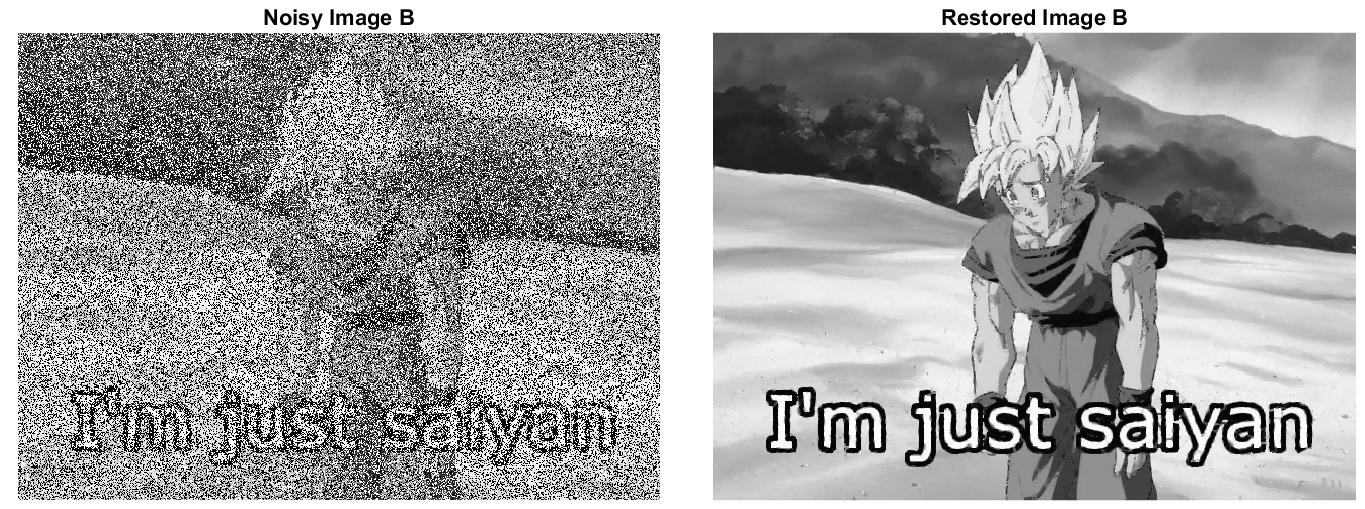
\includegraphics[width=16cm, height=6cm]{2.png}
  \caption{\small Total Variation inpainting applied on a grayscale image with salt \& pepper noise.}
\end{figure}

\end{document}
